% Diagram of Android activity life cycle
% Author: Pavel Seda 
\documentclass[border=10pt,11pt]{standalone}
\usepackage{tikz}
\usetikzlibrary{arrows.meta,arrows}
\usetikzlibrary{calc,decorations.markings}


\begin{document}   
% Drawing part, node distance is 1.5 cm and every node
% is prefilled with white background
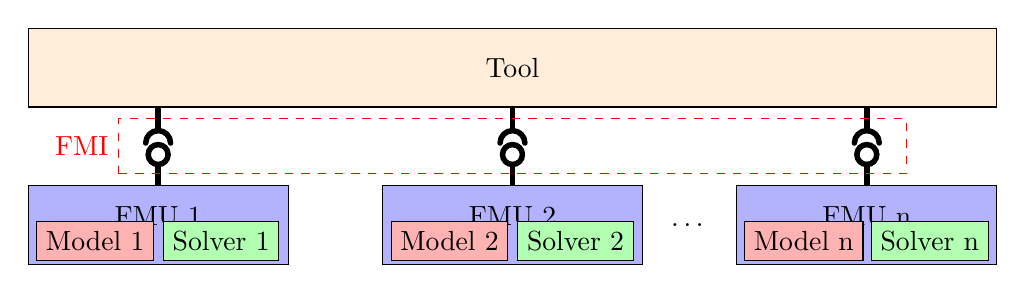
\begin{tikzpicture}[node distance=1.5cm,
    every node/.style={fill=white}, align=center]
		\tikzset{%
  >={Latex[width=2mm,length=2mm]},
  % Specifications for style of nodes:
            base/.style = {rectangle, draw=black,
                           minimum width=4cm, minimum height=1cm,
                           text centered},
  fmu/.style = {rectangle, draw=black,fill=blue!30,
                           minimum width=3.3cm, minimum height=1cm,text height=-0.40cm},
       model/.style = {rectangle, draw=black,fill=red!30,minimum width=1.3cm,minimum height=0.5cm},
    solver/.style = {rectangle, draw=black,fill=green!30,minimum width=1.3cm, minimum height=0.5cm},
         tool/.style = {rectangle, draw=black, fill=orange!15,
                          minimum width=12.3cm, minimum height=1cm},
				 FMI/.style = {rectangle,draw=red,dashed,fill=none,minimum width=10cm, minimum height=0.7cm},
}
  % Specification of nodes (position, etc.)
  
  
  \node (fmu1) [fmu] {FMU 1};
  \node (fmu2)  [fmu, right of=fmu1, xshift=3cm] {FMU 2};
	
	\node (fmu3)  [fmu, right of=fmu2, xshift=3cm] {FMU n};
	
	\node (tool) [tool, above of=fmu2, yshift=0.5cm] {Tool} ;
	
	
	\node (model1) [model, below of=fmu1, yshift=1.3cm,xshift=-0.8cm] {Model 1} ;
	\node (solver1) [solver,  below of=fmu1, yshift=1.3cm,xshift=0.8cm] {Solver 1} ;
	\node (model2) [model, below of=fmu2, yshift=1.3cm,xshift=-0.8cm] {Model 2} ;
	\node (solver1) [solver,  below of=fmu2, yshift=1.3cm,xshift=0.8cm] {Solver 2} ;
	\node (model3) [model, below of=fmu3, yshift=1.3cm,xshift=-0.8cm] {Model n} ;
	\node (solver1) [solver,  below of=fmu3, yshift=1.3cm,xshift=0.8cm] {Solver n} ;
	
	
	
  %\node (white1) [rectangle,above of=fmu1, yshift=0.625cm,minimum width=0.5cm,minimum height=0.5cm]
     
  % Specification of lines between nodes specified above
  % with aditional nodes for description 
\path (fmu2) -- node[auto=false]{\ldots} (fmu3);
%\draw[-{Circle[open,length=0.4cm,width=0.4cm]},line width=0.7mm] (fmu1) -- ([yshift=0.7cm]fmu1.north); 
\draw[-o,line width=0.7mm] (fmu1) -- ([yshift=0.55cm]fmu1.north);
\draw[-o,line width=0.7mm] (fmu2) -- ([yshift=0.55cm]fmu2.north);
\draw[-o,line width=0.7mm] (fmu3) -- ([yshift=0.55cm]fmu3.north);

\draw[-{Arc Barb[reversed,round]},line width=0.7mm] ([yshift=1.0cm]fmu1.north) -- ++(0,-0.5);
\draw[-{Arc Barb[reversed,round]},line width=0.7mm] ([yshift=1.0cm]fmu2.north) -- ++(0,-0.5);
\draw[-{Arc Barb[reversed,round]},line width=0.7mm] ([yshift=1.0cm]fmu3.north) -- ++(0,-0.5);

\node (fmi) [FMI,above of=fmu2, yshift=-0.5cm,label={[text=red]west:FMI}] {} ;


  \end{tikzpicture}
\end{document}